\documentclass[english,a4paper,hidelinks,pdftex, 11 pt, class=report,crop=false]{standalone}
\usepackage[T1]{fontenc}
\usepackage[utf8]{luainputenc}
\usepackage{geometry}
\setlength{\parindent}{0bp}
\usepackage{import}
\usepackage[subpreambles=false]{standalone}
\usepackage{amsmath}
\usepackage{amssymb}
\usepackage{esint}
\usepackage{babel}
\usepackage{tabu}
\usepackage{lmodern}
\usepackage[dvipsnames]{xcolor}
\geometry{verbose, inner=2.3cm, outer=1.8 cm, bmargin=2cm, tmargin=1.8cm}
% Lister med bokstavar
\usepackage{enumitem}

\newcommand{\os}{\\[5pt]}
\newcommand{\vsk}{\\[12pt]}
\newcommand{\net}[2]{{\href{#1}{\color{blue}#2}}}

\usepackage{bm}

\usepackage{hyperref}


\usepackage[many]{tcolorbox}
\newcommand{\reg}[2][]{\begin{tcolorbox}[boxrule=0.3 mm,arc=0mm,colback=blue!3] {\Large \textbf{#1} \vspace{5 pt}}\newline #2  \end{tcolorbox}\vspace{-5pt}}

\newcommand\eks[2][]{\begin{tcolorbox}[boxrule=0.3 mm,arc=0mm,enhanced jigsaw,breakable,colback=green!3] {\Large \textbf{Eksempel #1} \vspace{5 pt}\\} #2 \end{tcolorbox}\vspace{-5pt} }

\newcommand{\asym}[1]{/home/sindre/G/fig/#1}
\newcommand{\fig}[1]{\begin{figure}
		\centering
		\includegraphics[]{\asym{#1}}
\end{figure}}

\newcommand{\ca}[1]{{\color{blue} #1}}
\newcommand{\cb}[1]{{\color{orange} #1}}
\newcommand{\cc}[1]{{\color{ForestGreen} #1}}
\newcommand{\cd}[1]{{\color{cyan} #1}}

\begin{document}
	\pagestyle{empty}
\large
\section*{\huge Lekser fredag matematikk veke 11}
\reg[Omkrinsen til ein sirkel]{
	Omkrinsen til ein sirkel er tilnærma lik
	\[ 3,14\cdot \text{diameter} \]
\begin{figure}
	\centering
	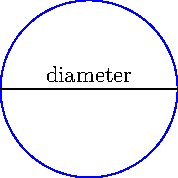
\includegraphics[]{sirkomkr}
\end{figure}
}
\eks[1]{
Finn omkinsen til sirkelen.
\begin{figure}
	\centering
	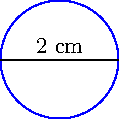
\includegraphics[]{sirkomkr2}
\end{figure}
\textbf{Svar}
\[ 3,14\cdot2 =6.28 \]
Omkrinsen til sirkelen er 6.28 cm.
}\vspace{20pt}
{\Large \textbf{Oppgåver}}\vsk
Mål diameteren med linjal, rund av til næraste heiltal (f. eks 2), og rekn ut omkrinsen til sirklane.\\
	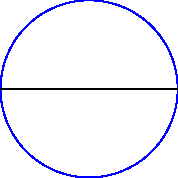
\includegraphics[]{sirkomkr3} \qquad
		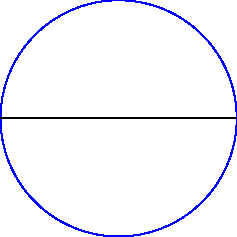
\includegraphics[]{sirkomkr4} \qquad
		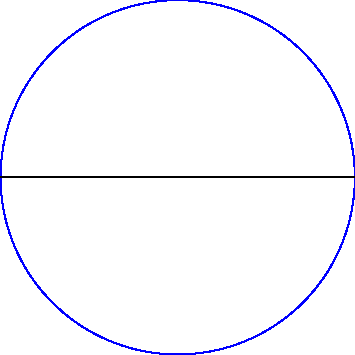
\includegraphics[]{sirkomkr6}
		\newpage
		\centering
		
\includegraphics[]{ruter}
\end{document}




